\documentclass[A4paper,11pt]{article}
\usepackage{graphicx}
\usepackage{eurosym}
\usepackage[latin1]{inputenc}
\usepackage[T1]{fontenc}
\usepackage[francais]{babel}
\usepackage{fancyhdr}
\pagestyle{fancy}

\title{\textbf{\Huge Cahier des charges}\\Projet : Quantum Quest\\ Groupe : Script Makers}
\author{Anthony TRUONG, Coralien TOSO,\\ L\'eo TORDJMAN, Damien RIOUAL}
\date{15 janvier 2016}

\fancyhead[C]{Cahier des charges : Quantum Quest}
\fancyhead[R]{ }
\fancyhead[L]{ }

\fancyfoot[R]{EPITA 2020}

\begin{document}
\maketitle
\begin{center}
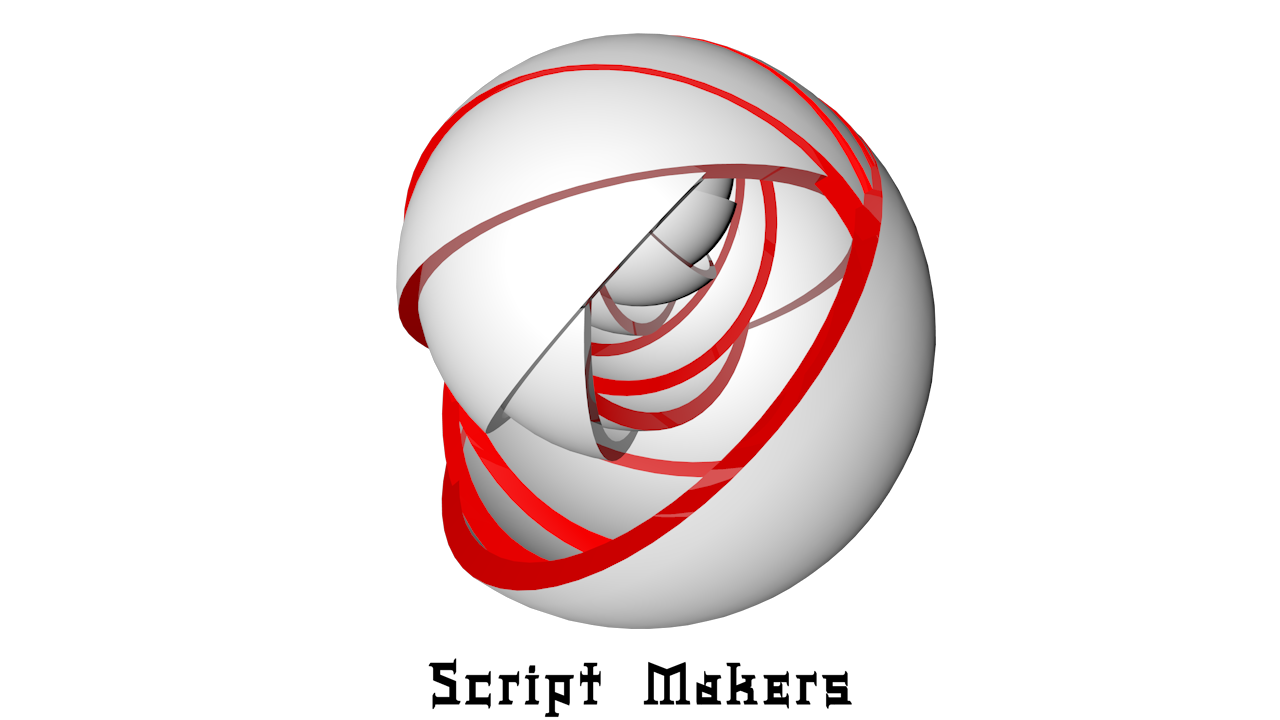
\includegraphics[scale=0.25]{logo.png}
\end{center}
\newpage
\tableofcontents
\newpage

\section{Introduction}
Voici le cahier des charges du projet Quantum Quest, r\'ealis\'e par le groupe Script Makers et constitu\'e de quatre membres : RIOUAL Damien, TORDJMAN L\'eo, TOSO Coralien et TRUONG Anthony.\\

Ce document aura ainsi pour but de vous pr\'esenter chacun des membres, leurs motivations, mais surtout notre projet, r\'ealis\'e \`a l'occasion de notre second semestre au sein de l'EPITA. Ainsi que les pr\'evisions, du groupe tout le long du d\'eveloppement de notre jeu vid\'eo.\\

Les membres de notre groupe jouent, de mani\`ere r\'eguli\`ere aux jeux vid\'eos, c'est pourquoi la r\'ealisation d'un jeu nous para\^it des plus attrayantes. Etant donn\'e que ce domaine nous est particuli\`erement familier, ce projet nous aidera \`a d\'ecouvrir ce qu'il se cache derri\`ere les divers ennemis que nous affrontons r\'eguli\`erement.\\

Le principal but de notre projet sera donc d'approfondir nos comp\'etences en programmation, ainsi que de renforcer notre travail en \'equipe (chose que nous ne pouvions pas forc\'ement travailler avant cette ann\'ee). En effet, la communication au sein de l'\'equipe sera cruciale afin de mener \`a bien notre jeu. Le travail en autonomie sera \'egalement de mise, et seront des moments durant lesquels chacun de nous d\'ecouvrira les diff\'erents logiciels pour sa part du projet.\\

\begin{center}
Bonne lecture !
\end{center}
\begin{center}

\includegraphics[scale=0.06]{epita_logo.png}
\end{center}
\newpage
\section{Pr\'esentation}

\subsection{Origine du projet}
Nous allons d\'esormais vous pr\'esenter d'o\`u nous est venue l'id\'ee de ce projet.\\

Les nouvelles technologies est un domaine de plus en plus pr\'esent dans la vie de tous les jours, suscitant ainsi notre int\'er\^et et notre pr\'esence \`a l'EPITA. Ce domaine \'etant un de nos principaux centres d'int\'er\^et, nous avons ainsi d\'ecid\'e de r\'ealiser un jeu vid\'eo sur ce th\`eme.\\
Le projet sera ainsi un RPG (jeu de r\^ole), \`a la troisi\`eme personne o\`u le joueur pourra incarner un personnage dont les sp\'ecificit\'es seront d\'etermin\'ees par un choix parmi les trois classes qu'il sera possible d'incarner dans le jeu. Le personnage \'evoluera dans un univers futuriste, en qu\^ete du tant d\'esir\'e processeur quantique.

\subsection{Les membres}
\subsubsection{Anthony TRUONG}
J'ai abord\'e l'id\'ee de ce projet avec quelques appr\'ehensions, notamment du fait qu'avant d'arriver \`a l'EPITA, je n'avais encore jamais cod\'e. N\'eanmoins, \`a l'aide de ce projet, je vais progresser \'enorm\'ement dans le domaine, que ce soit en programmation, en d\'ecouvrant de diff\'erent langages, tels que le html, css, php ou encore le java script, afin de r\'ealiser un site-web.

\subsubsection{Coralien TOSO}
Avant de rejoindre l'EPITA j'ai pu participer \`a l'\'elaboration d'un petit logiciel pour pc ainsi qu'\`a de la mod\'elisation et animation 3D. Mais jamais de jeux video, donc je suis content de pouvoir participer \`a cette nouvelle experience. Ce projet va me permettre de d\'evelopper mes comp\'etences en programmation ainsi qu'en conception graphique. Cr\'eer un jeu video en groupe va me permettre d'am\'eliorer mon auto-discipline et ma capacit\'e \`a travailler en groupe.
\newpage

\subsubsection{L\'eo TORDJMAN}
J'ai toujours grandement appr\'eci\'e de pouvoir observer mes id\'ees se concr\'etiser. Quoi de mieux pour cela qu'un jeu vid\'eo ? Ce projet me permettra donc d'apprendre le travail en \'equipe - notamment l'utilisation de Git - , de d\'ecouvrir le moteur de jeu Unity, ainsi qu'approfondir mes connaissances du C\#. Et surtout... qui n'a jamais r\^ev\'e de faire son propre jeu vid\'eo ?
\subsubsection{Damien RIOUAL}
Etant int\'eress\'e par l'informatique, la r\'esolution de probl\`emes algorithmiques et par la s\'ecurit\'e informatique, j'ai voulu int\'egrer l'EPITA il y a quelques temps afin d'apprendre de nouvelles choses \`a ce sujet car cela m'int\'eresse beaucoup. Le fait de faire ce projet me permettra d'obtenir une bonne experience du travail de groupe et d'acqu\'erir de nouvelles connaissances dans les logiciels que nous utiliserons tels que Unity, Blender ainsi qu'en LaTeX et plus g\'en\'eralement dans l'informatique. Je suis motiv\'e \`a r\'ealiser mon premier projet en \'equipe.

\section{Gameplay}
\subsection{Histoire}
Dans un univers o\`u les avanc\'ees technologiques permettent aux machines de se comporter et de se d\'eplacer au m\^eme titre que les humains, la course \`a la technologie quantique est plus que jamais pr\'esente. 

Cependant, la libert\'e de circulation des Intelligences Artificielles provoque la r\'ebellion de certains humains : les Ind\'ependantistes. Ces rebelles exploiteront des Intelligences Artificielles d\'efectueuses et en pirateront d'autres, afin de revenir \`a un monde appartenant exclusivement aux Hommes. 

Infiltr\'ees parmi ces derniers, certaines Intelligences Artificielles veulent juste tout d\'etruire (mode Terminator).

Quantum Quest est un RPG du m\^eme style que World of Warcraft, Starwars the Old Republic, ou encore TERA Online.
\newpage
\subsection{Personnages}
Le joueur pourra incarner un personnage, une Intelligence Artificielle, au choix parmi les 3 classes que nous vous pr\'esenterons ci-dessous.
\subsubsection{Server}
Les Servers, autrefois peu connus du grand public, s'illustrent d\'esormais comme \'etant les protecteurs de leurs alli\'es gr\^ace \`a leur taille imposante et leur robustesse \`a toute \'epreuve.

Cette classe incarne les Tanks \`a l'\'etat pur. Ces personnages poss\`edent une vie importante ainsi qu'une bonne d\'efense, mais une attaque et une vitesse r\'eduites. Ils ont un syst\`eme d'attaques bas\'e sur la protection de ses alli\'es et de lui-m\^eme, ainsi que sur les effets de contr\^oles.
\begin{center}
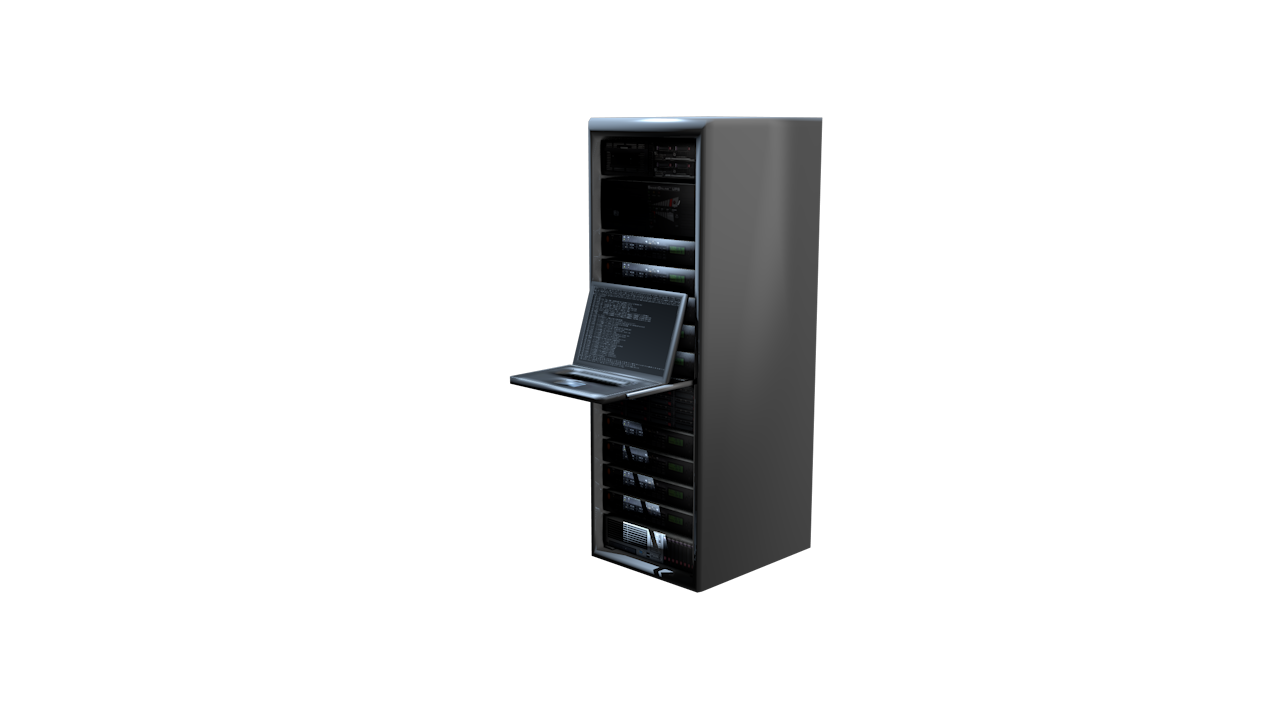
\includegraphics[scale=0.25]{sever.png}
\end{center}
\subsubsection{Computer}
Les Computers, contrairement aux Servers, \'etaient connus de tous et quasiment indispensables pour chaque personne. Aujourd'hui, frustr\'es qu'on les compare sans cesse aux Laptops plus "passe-partout" qu'eux, ils se sont renferm\'es sur eux m\^eme afin d'accro\^itre leur puissance et de peaufiner des scripts destructeurs.

La classe Computer repr\'esentent les DPS "lourds". Ils infligent des d\'eg\^ats \'elev\'es et ma\^itrisent des attaques puissantes pour achever l'ennemi.
\begin{center}
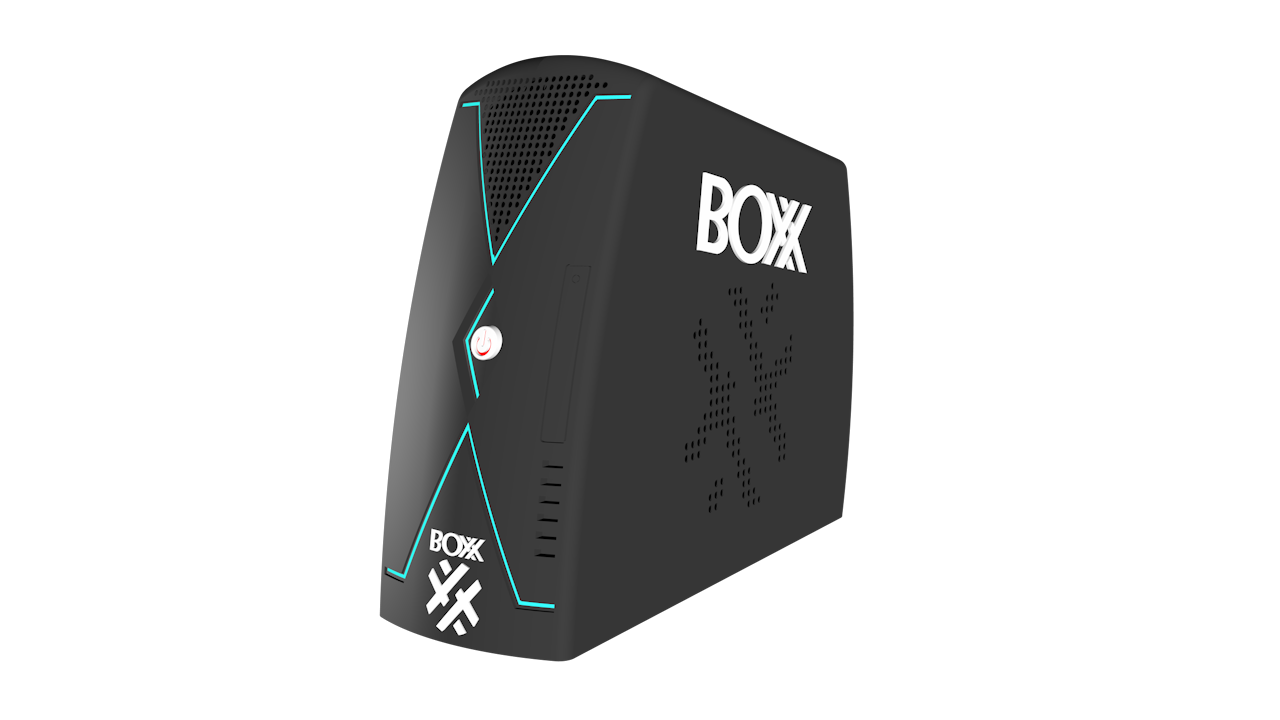
\includegraphics[scale=0.2]{computer.png}
\end{center}
\subsubsection{Laptop}
Enfin les Laptops, petits derniers de l'industrie des ordinateurs encore pr\'esents aujourd'hui, repr\'esentent les "blonds" des Intelligences Artificielles. Toujours plus fins et plus rapides, ils tailladent leurs ennemis, ne se souciant que d'eux m\^eme.

La classe Laptop correspond aux DPS "l\'egers". Ils ont moins de vie que les autres classes, mais foudroient leurs ennemis en encha\^inant les attaques \`a la m\^eme vitesse que l'\'electricit\'e parcourt leurs circuits.
\begin{center}
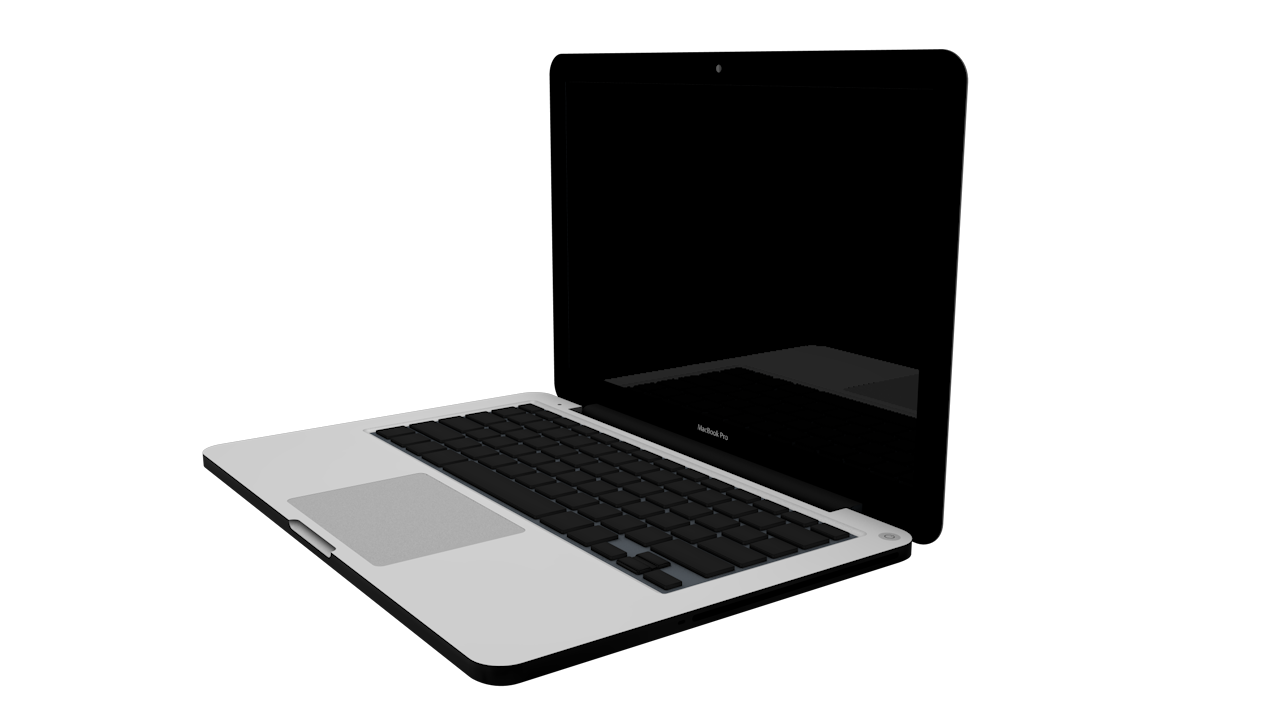
\includegraphics[scale=0.2]{laptop.png}
\end{center}
\newpage
\subsection{Quantum Quest}
Le but du jeu sera de d\'ecouvrir le mythique processeur quantique, et de cette mani\`ere devenir l'Intelligence Artificielle la plus puissante et soumettre ses ennemis. Et surtout S'ECLATER :) !!!

Pour y parvenir, le joueur parcourra son environnement en compl\'etant diverses qu\^etes. Ces qu\^etes leur permettront d'acqu\'erir de l'exp\'erience et de l'argent afin d'am\'eliorer ses comp\'etences et ses composants.


\section{D\'ecoupage du projet}

\subsection{Les scripts}
Pour notre jeu, nous r\'ealiserons les scripts en C\# \`a l'aide de Visual Studio, puis nous les importerons dans Unity.
Les scripts concerneront l'implementation des classes, la mise en r\'eseau, ainsi que la gestion de l'interface graphique.
Cette partie du projet va ainsi \^etre g\'er\'ee par deux membres, RIOUAL Damien et TORDJMAN L\'eo.
\subsection{Les mod\`eles 3D}
La partie graphique du jeu, soit, la mod\'elisation, l'animation des mod\`eles 3D, et \'egalement les menus du jeu, vont \^etre r\'ealis\'es \`a l'aide de diff\'erents logiciels, tel que Photoshop CS6, Blender, ou encore Cinema 4D, tout cela va essentiellement \^etre r\'ealis\'e par TOSO Coralien.
\subsection{Le son}
Que serait un jeu vid\'eo sans son ? Pas grand chose. En effet, cet \'el\'ement est particuli\`erement important, cela permet au joueur de s'immerger dans le jeu et faire partie int\'egrante de l'action s'y d\'eroulant. L'environnement sonore du jeu sera ainsi compos\'e de divers bruitages, et de musiques.

La r\'ealisation de l'ambiance sonore, va alors \^etre partag\'ee entre TOSO Coralien, et TRUONG Anthony, \`a l'aide d'Audacity et d'une table de mixage.
\newpage
\subsection{Le site}
Le site web est une fa\c{c}ade importante de notre projet : il repr\'esente le c\^ot\'e marketing de celui-ci. C'est pour cela que nous nous devons de bien soigner l'aspect graphique. Le site nous permettra donc de promouvoir notre jeu vid\'eo mais \'egalement d'avoir un point de contact entre les utilisateurs et notre groupe.

Cette partie sera r\'ealis\'ee par TRUONG Anthony. Nous envisageons l'utilisation du HTML, PHP et du CSS.
\subsection{Le r\'eseau}
Afin d'am\'eliorer la qualit\'e de notre jeu, nous impl\'ementerons un mode multi-joueurs car il est beaucoup plus sympa de jouer contre des amis plut\^ot que contre des Intelligences Artificielles. De plus, la base de la programmation de tout r\'eseau est bas\'ee sur les sockets.
Dans cette optique, la mise en place du r\'eseau sera assur\'ee par RIOUAL Damien et TORDJMAN L\'eo.

\section{R\'epartition des t\^aches}
Voici la r\'epartition des diff\'erentes t\^aches. Nous avons choisi cette r\'epartition des t\^aches en fonction de nos go\^uts, nos pr\'erequis ainsi que celles qui nous correspondaient le plus.\\
\begin{center}
\begin{tabular}{|c|c|c|c|c|}
\hline
T\^aches : & Anthony & Coralien & Damien & ~~L\'eo~~~\\
\hline
Scripts &   &   & X & X\\
\hline
Gameplay &   &   & X & X\\
\hline
Mod\`eles 3D &   & X &   &  \\
\hline
GUI* & X & X  &  & \\
\hline
Son & X & X &   &  \\
\hline
Site Web & X &   &   &  \\
\hline
Rapport LaTeX & X & X & X & X\\
\hline
R\'eseau & & & X & X\\
\hline
\end{tabular}\\
\end{center}
GUI* = Interface graphique
\begin{center}
\section{Planning}
\begin{tabular}{|c|c|c|c|c|c|c|}
\hline
 & Gameplay & Mod\`eles 3D & GUI & Son & Site Web & R\'eseau\\
\hline
Premi\`ere soutenance & 20\% & 30\% & 10\% & 30\% & 20\% & 10\%\\
\hline
Deuxi\`eme soutenance & 60\% & 50\% & 50\% & 65\% & 50\% & 50\%\\
\hline
Derni\`ere soutenance &100\% & 100\% & 100\% & 100\% & 100\% & 100\%\\
\hline
\end{tabular}
\end{center}
\subsection{Premi\`ere soutenance}
Pour la premi\`ere soutenance, l'\'equipe Script Makers souhait\'e impl\'ementer dans son projet Quantum Quest la possibilit\'e d'\'evoluer avec un personnage dans une salle, faisant office de salle de d\'epart. Ce personnage poss\`edera quelques animations de base, telles que le d\'eplacement \`a vitesse normale et le d\'eplacement rapide ainsi que le saut.\\ 
\subsection{Deuxi\`eme soutenance}
Pour la deuxi\`eme soutenance, le projet Quantum Quest sera d\'ej\`a plus abouti. L'\'equipe Script Makers impl\'ementera un syst\`eme d'inventaire ainsi qu'un syst\`eme d'attaques et de JcE (Joueur contre Environnement), un environnement avec quelques \'el\'ements de d\'ecor, une ambiance sonore ainsi qu'une partie r\'eseau avec du multi-joueurs. Pour cette soutenance un site web sera accessible. Sur ce site il y aura une pr\'esentation de l'\'equipe ainsi que du projet.\\
\subsection{Derni\`ere soutenance}
Lors de l'ultime soutenance, le projet Quantum Quest sera totalement abouti. Il int\'egrera la possibilit\'e de choisir la classe que le joueur souhaitera incarner. Un syst\`eme de d\'eplacement, d'inventaire et de qu\^etes plus pouss\'e. Il y aura \'egalement un menu d'options, et une ambiance sonore plus d\'evelopp\'ee avec des musiques d'ambiance. Le syst\`eme multi-joueurs permettra aux diff\'erents joueurs d'interagir entre eux. Le site web permettra de t\'el\'echarger la version termin\'ee de projet.\\

\section{Moyens Mat\'eriels et Intellectuels}

\subsection{Mat\'eriel}
Voici le mat\'eriel dont nous disposons pour r\'ealiser le projet :\\
\begin{center}
\begin{tabular}{|c|c|c|c|c|}
\hline
 & Processeur & Carte Graphique & M\'emoire Vive\\
\hline
Anthony & Intel Core i7-5500U & NVIDIA GeForce 940M & 6Go \\
\hline
Coralien & Intel Core i7-4820k & NVIDIA GeForce GTX 880M & 32Go \\
\hline
Damien & Intel Core i7 & AMD Radeon R9 M370X & 16Go \\
\hline
L\'eo & Intel Core i7-4820k & NVIDIA GeForce GTX 660 & 8Go \\
\hline

\end{tabular}
\end{center}
\subsection{Logiciels et Ressources}
Pour faire ce projet nous utiliserons principalement le logiciel Unity pour tout ce qui est des d\'eplacements des personnages. Pour les \'el\'ements graphiques nous utiliserons les logiciels Cinema 4D, Photoshop CS6 et Blender. Et pour tout ce qui est du code et des scripts nous utiliserons Visual Studio.
Pour r\'ediger les rapports en LaTeX nous utiliserons le Guide de Didier Verna distribu\'e en d\'ebut d'ann\'ee ainsi qu'un tutoriel LaTeX sur le site OpenClassrooms.

\subsubsection{Co\^ut}
\begin{center}
\begin{tabular}{|c|c|c|c|}
\hline
Logiciel & Editeur & Type & Prix\\
\hline
Visual Studio & Microsoft & IDE* & 0 \euro\\
\hline
Unity & Unity Technologies & Moteur de jeu & 0 \euro\\
\hline
Brackets & Adobe Systems & Texte & 0 \euro\\
\hline
Cinema 4D & Maxon & Mod\'elisation 3D & 900 \euro\\
\hline
Photoshop CS6 & Adobe &  DAO* & 800/1200 \euro\\
\hline
Blender & La Fondation Blender & Mod\'elisation 3D & 0 \euro\\
\hline
Audacity & Audacity & Son & 0 \euro\\
\hline
LaTeXShop & LaTeX & Texte & 0 \euro\\
\hline
\end{tabular}\\
\end{center}
IDE* = Environnement de d\'eveloppement int\'egr\'e
DAO* = Dessin Assist\'e par Ordinateur

\section{Conclusion}
Vous voici d\'esormais \`a la fin de ce cahier des charges, mais ceci n'est qu'un d\'ebut. Les bases ont ainsi pu \^etre d\'efinies. Alors il ne restera aux Script Makers qu'\`a r\'ealiser ce projet pharaonique dans les temps, et \`a faire face aux difficult\'es. Cette exp\'erience ne pourra que nous rendre meilleurs, et tester les limites de chacun.

Nous nous soutiendrons dans ce premier projet afin d'avoir le meilleur projet possible et d'en tirer le meilleur de nos capacit\'es. 

\end{document}
